






\section{Background} \label{s:background}

There are numerous game engines with their associated development environments which could be suitable for CAV development, e.g. Unreal, Unity, CryEngine. Specific autonomous driving research tools have been created to abstract and simplify the development environment, some of which are based on existing engines, e.g. Carla, AirSim, Apollo, and some have been developed specifically, e.g. the could based Nvidia Drive Constellation simulator. \TODO{ref each of these}

Investigating the determinism of gaming engines has not attracted much research interest since performance is more critical for playing games than accurate and repeatable runtime execution. However, when these engines are used for CAV development then deterministic behaviour is required. This section gives an overview of a gaming engine and what sources or settings in the engine may affect \textit{simulation variance}.
%
% \noindent This section overviews important information and concepts in physics engines, which are relevant to their usage in CAV simulations. Particularly, on how physics engines operate and the sources of non-determinism in these engines necessary to understand the contribution of this paper.

% ======= Overview of a Game Loop
\subsection{Overview of a Game Loop} \label{GameLoopSection}
The game loop is responsible for the interaction between the maths, physics and rendering engines. Figure \ref{GameEngineLoopDiagram} depicts a basic representation of the process flow in a game engine loop. A game loop is broken up into three distinct phases: processing the inputs, updating the game world (Physics Engine), and generating outputs (Rendering).~\cite{GameEngineArchBook}

\begin{figure}[h]
\centering
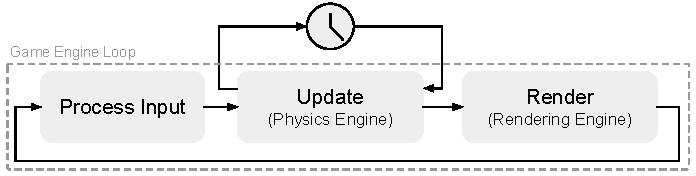
\includegraphics[width=0.5\textwidth]{Other/Figures/GameEngineLoop.pdf}
\caption{Game engine loop block diagram~\cite{GameProgPatternsBook}}
\label{GameEngineLoopDiagram}
\end{figure}
The first part of the game loop is to process the user inputs which may take the form of user keyed inputs or, in the case of CAV development, the resultant actions of the autonomous vehicle given the current state of the environment. For example, the throttle and braking inputs from the PID controller controlling the speed of an AV. %\TODO{For AG: need to expand, e.g what are the inputs?} %\TODO{For AG: does game logic need to be mentioned?}
%
The update interprets the intended actions of all dynamic actors in the scene, performs any necessary physics calculations and updates the actor states. %This update process can still proceed independelty of the main game loop as symbolised by the clock in the upper loop in Figure~\ref{GameEngineLoopDiagram}. % \TODO{For AG: what does the clock symbolise, need to explain it?}
%
The rendering engine then takes the updated actor states and renders the scene~\cite{GameProgPatternsBook}. %\TODO{For AG: you cite this book 4 times which might be too much as a general reference, is there something specific you want to draw the reader towards in the book? What specifically about the rendering part of this cycle does the book help to illustrate the point?}

It is necessary to have an understanding of how rendering and physics engines operate together in order to grasp some of the sources of non-determinsim that will be mentioned. %\TODO{For AG: why is this crucial and can we say that we resolved it if it is crucial?}
The game loop operates as follows: (see Figure \ref{GameEngineLoopDiagram})
\begin{itemize}[leftmargin=*]
    \item At the beginning of each tick (scene), the lag between the game clock and the real world is updated based on how much real time passed. This measures how far the game's clock is behind compared to the real world.
    \item Then the user inputs are processed.
    \item There is then an inner loop to update the physics engine (clock symbol in Figure~\ref{GameEngineLoopDiagram}), incrementing at fixed step until the game clock is equal to the real world. The physics engine uses a fixed time step, because it makes everything simpler and more stable for physics and AI. The shorter this fixed time step is, the more processing time it takes to catch up to real time and the more deterministic the engine becomes and vice versa, as will be explained in section \ref{s:nondeterminisimSources}. Thus, ideally the time step should be as short as possible, so that simulations run with high fidelity on fast machines. However, if the fixed time step is too short i.e. less than the time it takes to process an ``Update" inner loop on some (slow) machines, then the simulation will simply never catch up on these slow machines.
    \item Rendering occurs once the physics engine catches up. The process then starts again.
\end{itemize} 



The time step, $dt$, in any physics calculation is important. To use a fixed physics time step the user's display refresh rate needs to be known in advance. This requires an update loop to take less than one frame of real world time~\cite{gaffer}. Given the different capabilities of game players hardware a variable delta time can be implemented taking the previous frame time as the next $dt$. However, variable $dt$ can lead to different physical results and in some cases unrealistic physics. Semi-fixed or limited frame rates ensure $dt$ does not exceed some user-defined limit to meet a minimum standard of physical representation but allows computational headroom for slower hardware. Some engines provide sub-stepping which does multiple physics calculations per frame at a greater CPU cost~\footnote{https://docs.unrealengine.com/en-US/Engine/Physics/Substepping/index.html}. If the engine tries to render between updates \textit{residual lag} can occur and extrapolation between frames is performed to smooth transition between scenes.%\cite{GameEngineArchBook}\cite{GameProgPatternsBook}



% This process allows hardware scalability, but the rendering will become of jerky quality on slower machines. These engines update at fixed intervals and render whenever they can, which is not steady. This results in what is so called residual lag\cite{GameEngineArchBook}\cite{GameProgPatternsBook}, where the engine is trying to render between two consecutive updates. In this case, the engine will use extrapolation techniques to give an estimate of where the object should be. This often is sufficient for gaming purposes and unnoticeable to the user, in fact it improves the stuttery motion.


\begin{figure*}[b]
    \centering
    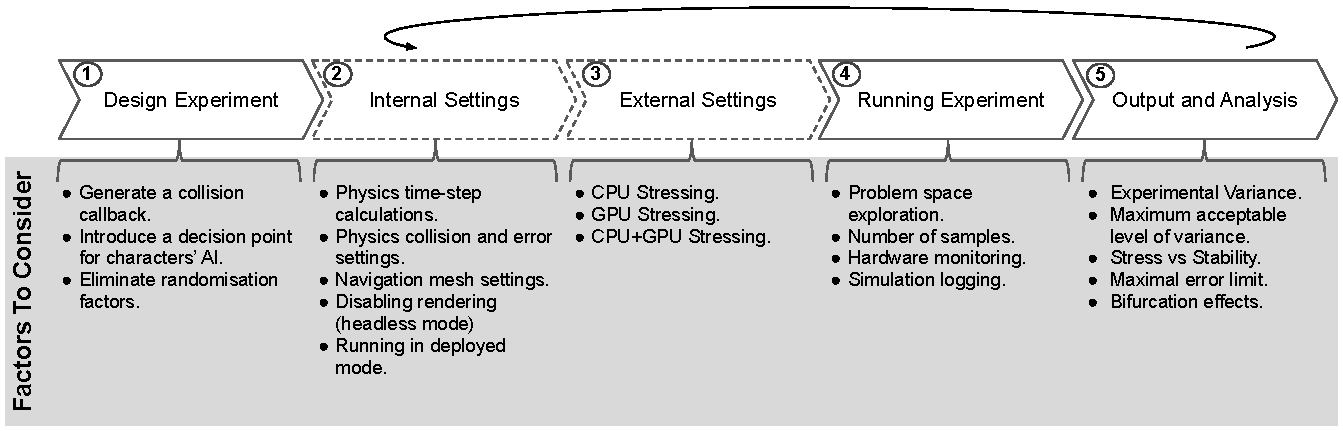
\includegraphics[width=0.99\linewidth]{Other/Figures/MethodologyDiagram.pdf}
    \caption{Shows a flow diagram of the methodology proposed to define the level of simulation variance of a gaming engine for usage in CAV simulations.}

    \label{method_diagram}
\end{figure*}

% ======= Sources of non-determinism
\subsection{Sources of non-determinism} \label{s:nondeterminisimSources}
\noindent After establishing an understanding of how physics engines work, the focus will now be on what causes these engines to be non-deterministic. 
The main reasons that we think are causes of these engines' non-determinism are discussed below. \\\\
%
\noindent\underline{\textit{Floating Points:}}
A generic issue with computers are floating points precision. 
Various errors occur when doing arithmetic manipulations using floating points, especially when operating between large and small numbers due to rounding, memory limitations and so forth.\cite{FloatingPointArithmeticArticle}\cite{FloatingPointsBook}.

Translating to the usage of CAV simulations in physics engines, this could result in many precision issues; for instance consider a simulation where the world is infinite and progressively  generated in the physics engine. 
After a few hundred meters, precision issues will start to occur due to the coordinates used in arithmetic cacluations getting bigger, and will get progressively worse the further from the origin the simulation gets. 
Such reasons would often make one rapidly jump to conclude that floating points are the cause of non-determinism of these engines. 
However, it is important to note that these precision issues should be referred to as incorrecctness and not non-determinisim. 
Since hardware is deterministic, then the same hardware should produce the same exact output for the same inputted data i.e. even if the output is incorrect due to floating point precision it should always be the same, given the same hardware.\\\\ 
%
% A generic issue with computers are floating points precision. 
%Various errors occur when doing arithmetic manipulations using floating points, especially when operating between large and small numbers due to rounding, memory limitations and so forth.\cite{FloatingPointArithmeticArticle}\cite{FloatingPointsBook}. 
%Translating to the usage of CAV simulations for V\&V in physics engines, this could result in many precision issues resulting in complex non deterministic behaviours.
%
% For instance, consider a simulation where the world is infinite and progressively  generated in the physics engine. 
% After a few hundred meters, precision issues will start to occur, and will get progressively worse the further from the origin the simulation gets. 
% This is due to the values of the coordinates being used in calculations are getting bigger and hence will not cope with small values that are critical for V\&V testing purposes. 
% A solution to this problem is perhaps every time the simulations moves 100 meters away from the origin the entire world will move by 100m in the opposite direction. Thus, avoiding getting into floating point issues.\cite{FloatingPointArithmeticArticle}
%
% There are many scenarios that could be addressed, and solutions to them will entirely depend on the characteristics of that specific scenario. There is no generalised solution for the floating problem, regardless of how good computers get there will always be a limitation. However, floating points as they stand could just be sufficient for V\&V testing purposes. Whenever they are not, smart solutions can be found to accommodate for these limitations.\\\\
%
\noindent\underline{\textit{Scheduling of threads:}} Scheduling of threads is believed to be the main reason for non-deterministic behaviour of game engines. Given the same hardware the output should always be the same, unless scheduling of the threads change i.e. the utilisation of hardware is manipulated differently each time. This would then result in non-deterministic behaviours especailly if it is combined with the floating point problem discussed earlier. 
To solve the scheduling of threads problem, one would have to control all of the threads during runtime, which is very involved. To achieve that one would need to replace or control the whole run-time system to allocate tasks to the same threads in the same order. This is beyond the sope of our work and will not be covered in this paper.\\\\
%
\noindent\underline{\textit{Physics and Rendering clocks:}}
The inherent way of how these physics engines operate (i.e.game loops) causes the engine to be non-deterministic. 
A follow up from section \ref{GameLoopSection}, these engines use a variable frame rate, which is good for hardware scalability but creates a challenge for the physics engine which works best with small fixed time steps. 
The problem of having a variable frame rate could also contribute to the non-deterministic behaviour of these engines, especially if put together with the scheduling of threads problem. That is to say, if the frame rate is allowed to vary then it has to be controlled to give the same variablity through out a given test in order for the test results to be repeatable. This issue might be of negligible significance if the frame rate is consistent and the time steps are small enough. \\\\
%
\noindent\underline{\textit{Navigation meshes and AI:}}
Game engines' often use navigation meshes for AI path planning. Some CAV simulator developers claim that the built-in physics engines' AI is non-deterministic\cite{CARLABenchmark}. 
The validity of this depends on what are the built in AI algorithms being used by the engine. 
Most of them tend to use the A* algorithm\cite{AStarBook}, which is an algorithm with deterministic behaviour if the environment is deterministic\cite{AirsimUnrealArticle}\cite{UnrealAIDocumentation}. 
Therefore, the determinism of the AI depends on the determinism of the engine and how its navigation meshes are created/modelled, their shape, granularity etc. It is interesting to note that changes can occur to meshes every time the simulation is loaded or if dynamically loading these navigation meshes as the simulation proceeds. This non-deterministic behaviour can be also resorted to the different scheduling of threads, hence giving variations in meshes everytime they are loaded.


